\documentclass{beamer}
% \usetheme{Madrid}
\setbeamertemplate{caption}[numbered]
% \setbeamertemplate{page number in head/foot}[framenumber]

\setbeamertemplate{frametitle}[default][left]
\setbeamercolor{page number in head/foot}{fg=black}
\setbeamerfont{page number in head/foot}{size=\small}

\setbeamertemplate{footline}[page number]

\usepackage{datetime}
\usepackage{amsmath}
\usepackage[brazil]{babel}

\title{Análise do protocolo \textit{Committeeless Proof-of-Stake}: em busca de um melhor ponto de operação}
\author{Vinícius Peixoto\inst{1} \and Marco Aurélio Amaral Henriques\inst{1}}
\institute{\inst{1} Faculdade de Engenharia Elétrica e de Computação (FEEC) - Unicamp}
\date{18 de Setembro de 2023}

\begin{document}
\frame{\titlepage}

\section{Introdução}
\subsection{O que são blockchains?}
\begin{frame}
\frametitle{O que são blockchains?}
\begin{itemize}
    \item Livro-razão distribuído, imutável, aberto e descentralizado
    \item Unidade básica de dados: \textbf{bloco}
    \item Blocos são criados em intervalos definidos de tempo: \textbf{rodada}
    \item Blocos são ligados matematicamente entre si
\end{itemize}

\begin{figure}
    \centering
    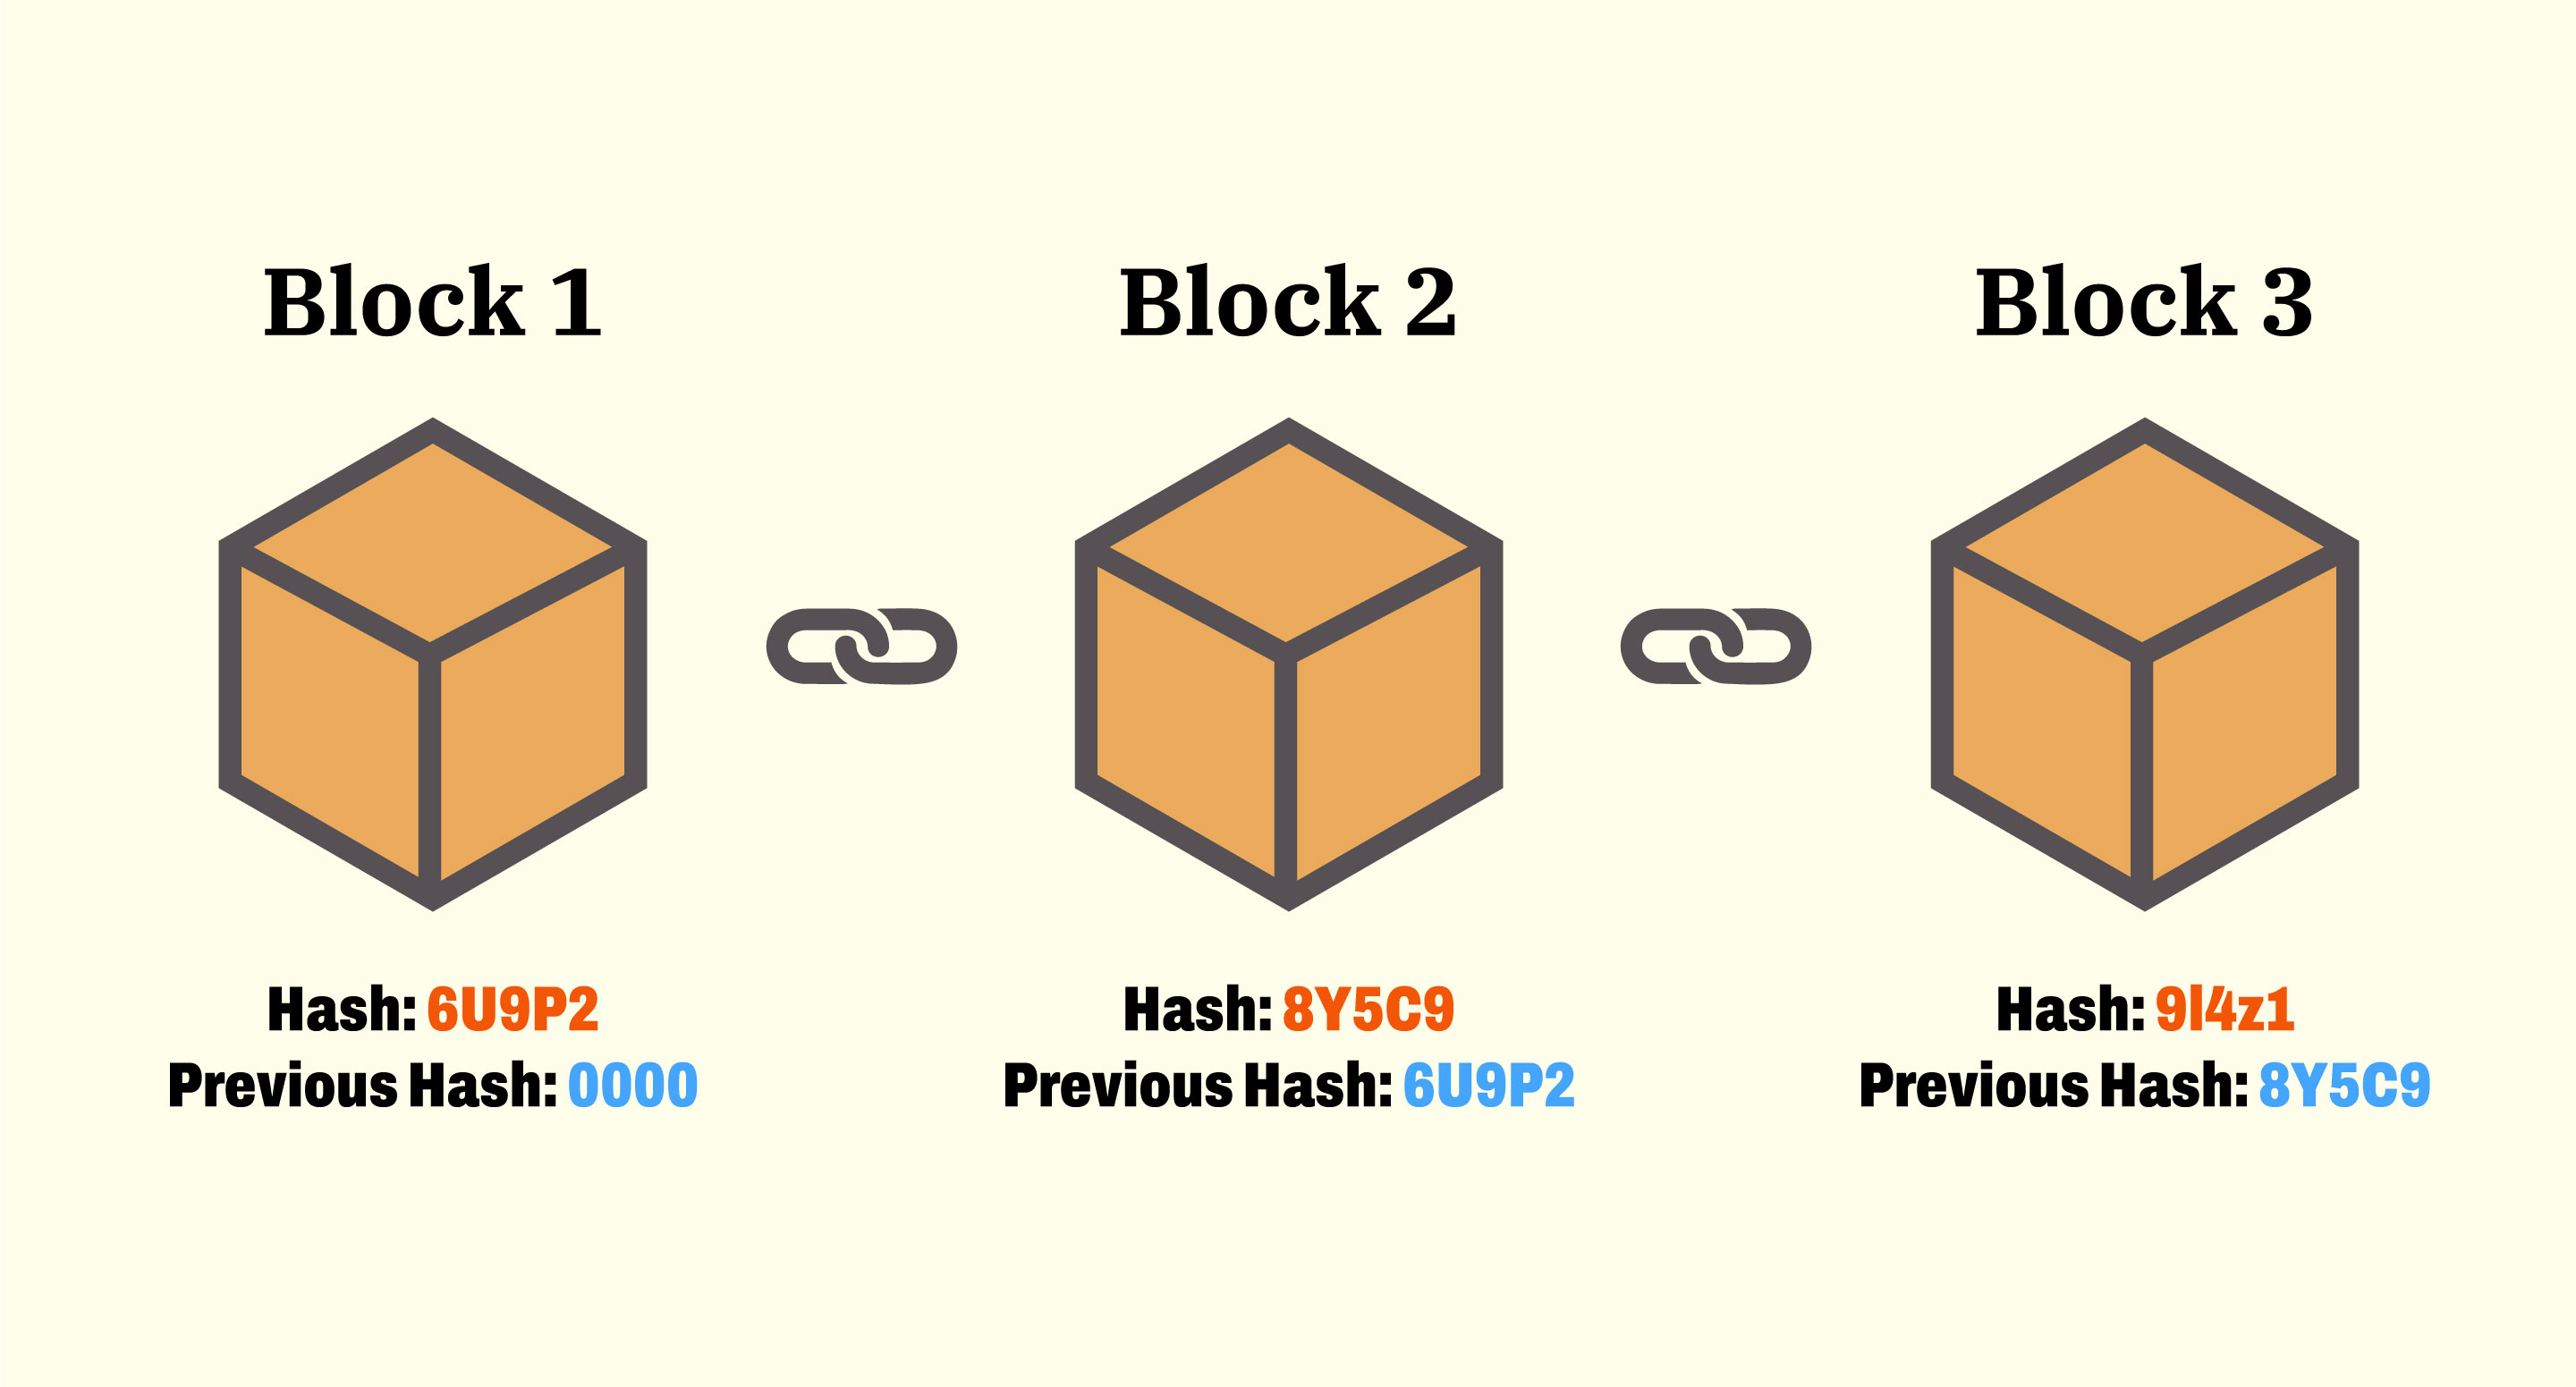
\includegraphics[width=0.6\textwidth]{images/blocks.jpg}
\end{figure}
\end{frame}

\begin{frame}
\frametitle{O que são blockchains?}
\begin{itemize}
    \item Blockchains como bancos de dados distribuídos: redes peer-to-peer
    \item Grande quantidade de nós na rede, porém \textbf{apenas um bloco por rodada}
    \item Necessidade de sincronização
    \item \textbf{Mecanismo de consenso distribuído}
\end{itemize}
\end{frame}

\subsection{Mecanismos de consenso}
\begin{frame}
\frametitle{Mecanismos de consenso}
Mecanismos mais utilizados:

\begin{itemize}
    \item Proof-of-Work: Bitcoin, Litecoin, Monero, ...
    \item Proof-of-Stake: Ethereum, BNB, Cardano, ...
\end{itemize}

Proof-of-Work (PoW):
\begin{itemize}
    \item Solução de um problema computacionalmente caro
    \item Quem resolver primeiro publica o bloco
    \item Grande desperdício de energia: trabalho de todos os nós exceto o sorteado é jogado fora
\end{itemize}
\end{frame}

\begin{frame}
\frametitle{Mecanismos de consenso}
Proof-of-Stake:
\begin{itemize}
    \item Alternativa mais energeticamente eficiente ao PoW
    \item Nós investem \textit{stake} para se tornarem \textbf{validadores}
    \item Validadores são sorteados para gerar blocos
    \item Validadores divididos em \textbf{comitês de votação}
    \item Comitês executam o protocolo de consenso e elegem blocos
\end{itemize}
\end{frame}

\begin{frame}
\frametitle{Mecanismos de consenso}
\begin{itemize}
    \item Problema:
    \begin{itemize}
        \item Centralização
        \item Comitês de validação são superfícies de ataque
    \end{itemize}
    \item Diversos ataques propostos: [Neuder 2021], [Schwarz-Schilling 2022]
    \begin{itemize}
        \item Estima-se que organizações com menos de 1/3 do stake consigam comprometer o consenso
    \end{itemize}
    \item Pergunta: é possível chegar ao consenso de forma \textbf{segura} e \textbf{descentralizada}?
\end{itemize}
\end{frame}

\section{O mecanismo CPoS}
\subsection{Visão geral}
\begin{frame}
\frametitle{O mecanismo CPoS}
Committeeless Proof-of-Stake (CPoS): 
\begin{itemize}
    \item Eliminação da necessidade de um comitê
    \item Trabalho de criação, propagação e validação
          de nós é completamente distribuído
    \item Rede tenta convergir para um consenso de forma totalmente distribuída
\end{itemize}
\end{frame}

\begin{frame}
    \frametitle{O mecanismo CPoS}
    \textbf{Este trabalho}: investigação preliminar da influência de parâmetros de configuração na segurança do protocolo
\end{frame}

\subsection{Mecanismo de sorteio}
\begin{frame}
\frametitle{Mecanismo de sorteio}
Sorteio determinístico:
\begin{itemize}
    \item Baseado no esquema Algorand [Gilad, 2017]
    \item Em um sorteio aleatório justo, seja $w_i$ o número de fichas (\textit{stake}) de um nó. Seja $p$ a chance de uma dada ficha ser sorteada. Então a chance de exatamente $k$ entre as $w_i$ fichas serem sorteadas é dada pela distribuição binomial:
        \begin{equation*}
            B(w_i, k, p) = \binom{w_i}{k} p^k (1-p)^{w_i - k}
        \end{equation*}
    \item Sorteio: a partir de um conjunto de hashes, é calculado um número $q \in [0.0, 1.0]$. O total de fichas sorteadas é o maior valor $k$ tal que $q > B(w_i, k, p)$.
\end{itemize}
\end{frame}

\begin{frame}
\frametitle{Mecanismo de sorteio}
\begin{figure}
    \centering
    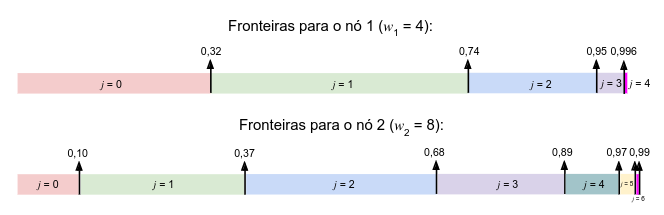
\includegraphics[width=\textwidth]{images/sortition.png}
    \caption{Subdivisão de intervalos para nós com stakes diferentes.}
\end{figure}
\end{frame}

\begin{frame}
\frametitle{Mecanismo de sorteio}
\begin{itemize}
    \item Seja $W = \sum w_i$ o \textit{stake} total na rede
    \item É possível provar que o número esperado \textbf{total de sorteios bem-sucedidos} por rodada é dado por $\tau = p \times W$
    \pause
    \item Parâmetro $\tau$: configura o número de blocos gerados por rodada
\end{itemize}
\end{frame}

\subsection{Confirmação de blocos}
\begin{frame}
\frametitle{Confirmação de blocos}
\begin{itemize}
    \item<1-> Processo probabilístico
    \item<2-> Nós estimam um nível de confiança para cada bloco não-confirmado
    \item<3-> Nível de confiança no bloco aumenta conforme chegam outros blocos
              que descendem dele
\end{itemize}
\end{frame}

\begin{frame}
\frametitle{Confirmação de blocos}
\begin{figure}
    \centering
    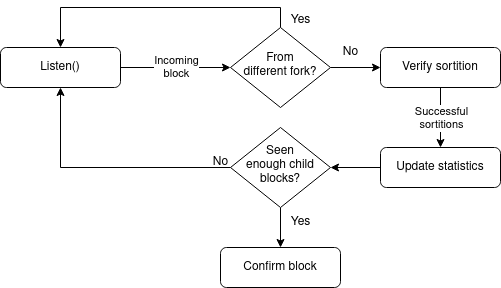
\includegraphics[height=0.6\textheight]{images/confirmation_fluxogram.png}
    \caption{Fluxograma do algoritmo de confirmação de blocos.}
\end{figure}
\end{frame}

\begin{frame}
\frametitle{Confirmação de blocos}
Mecanismo de confirmação: exige recebimento de blocos

\begin{itemize}
    \item<1-> Parâmetro $\tau$ controla o número total de blocos gerados
    \item<2-> Possível ataque: nós desonestos não divulgam blocos
    \item<3-> \textbf{Investigação deste trabalho}: influência de $\tau$ na performance e segurança da rede

\end{itemize}
\end{frame}

\section{Resultados parciais}
\subsection{Metodologia}
\begin{frame}
\frametitle{Experimentos}
\begin{itemize}
    \pause
    \item Experimento 1: influência de $\tau$ em uma rede saudável
    \begin{itemize}
        \item 25 peers no total
        \item Cada peer conhece outros 5 peers aleatórios
        \item Peers honestos (divulgam blocos)
    \end{itemize}
    \pause
    \item Experimento 2: influência de $\tau$ em uma rede desonesta
    \begin{itemize}
        \item 30 peers no total
        \item 5 deles ($\approx$ 16\%) não divulgam nós (desonestos)
        \item Topologia de rede conexa
    \end{itemize}
\end{itemize}
\end{frame}

\begin{frame}
\frametitle{Experimentos}
\begin{itemize}
    \item 50 rodadas no total
    \item Média ao longo de 10 repetições de cada experimento
    \item Nós geram blocos vazios (somente headers)
    \item Infraestrutura de Docker, rodando no Linux 6.4, AMD Ryzen 7 3700X, 32GB RAM
    \item Código disponível em \url{https://github.com/regras/cpos_v2}
\end{itemize}
\end{frame}

\subsection{Resultados}

\begin{frame}
\begin{figure}
\frametitle{Resultados}
    \centering
    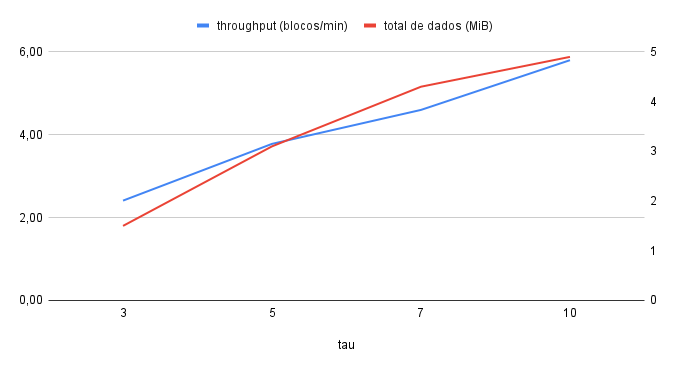
\includegraphics[width=0.8\textwidth]{images/test_honest_throughput_data.png}
    \caption{Influência de $\tau$ numa rede CPoS honesta.}
\end{figure}
\end{frame}
    
% \begin{frame}
% \begin{figure}
% \frametitle{Resultados}
%     \centering
%     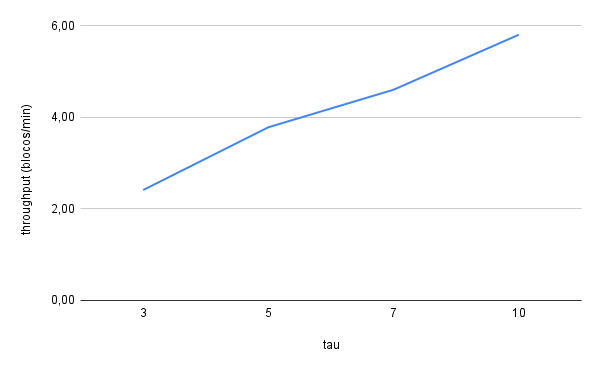
\includegraphics[width=0.8\textwidth]{images/test_honest_throughput.png}
%     \caption{Influência de $\tau$ no \textit{throughput} (blocos/min) da rede CPoS honesta}
% \end{figure}
% \end{frame}
%
% \begin{frame}
% \begin{figure}
% \frametitle{Resultados}
%     \centering
%     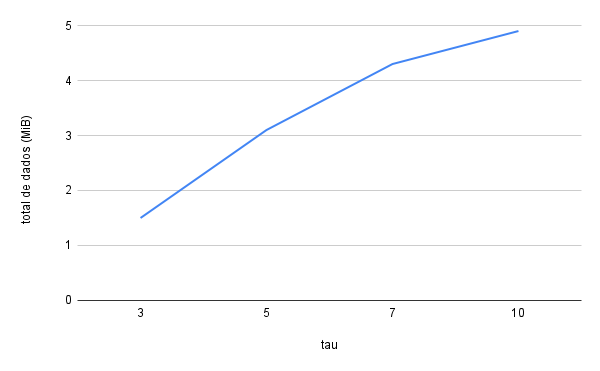
\includegraphics[width=0.8\textwidth]{images/test_honest_data_usage.png}
%     \caption{Influência de $\tau$ no volume de dados na rede CPoS}
% \end{figure}
% \end{frame}

\begin{frame}
\begin{figure}
\frametitle{Resultados}
    \centering
    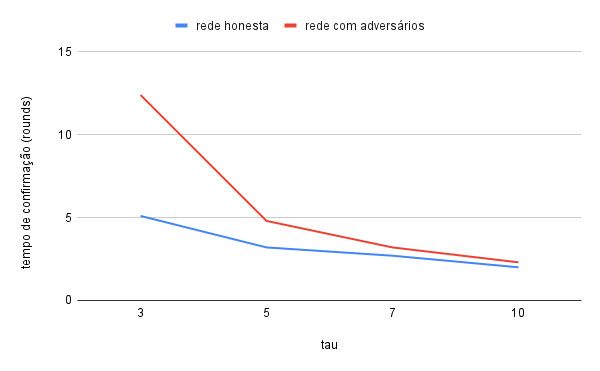
\includegraphics[width=0.8\textwidth]{images/test_adversarial.png}
    \caption{Influência de $\tau$ no tempo de confirmação do CPoS em uma rede saudável vs. uma rede adversarial}
\end{figure}
\end{frame}

\section{Conclusões e trabalhos futuros}
\subsection{Conclusões}
\begin{frame}
\frametitle{Conclusões}
\begin{itemize}
    \item Aumento de $\tau$:
    \pause
        \begin{itemize}
            \item<1-> Maior throughput, menor tempo de confirmação
            \item<2-> Aumento da resiliência em presença de nós desonestos
            \item<3-> Contudo: aumento significativo no número de mensagens e total de dados em circulação
        \end{itemize}
    \item<4-> Necessidade de encontrar um equilíbrio entre o valor de $\tau$ e o impacto na rede
        \begin{itemize}
            \item<5-> Envio somente de headers até que a rede escolha um bloco; somente então divulgação de blocos ocorre
        \end{itemize}
\end{itemize}
\end{frame}

\begin{frame}
\frametitle{Conclusões}
Trabalhos futuros:
\begin{itemize}
    \item Polimentos e melhorias na implementação atual do CPoS
    \item Execução de testes mais extensivos (maior número de blocos, nós distribuídos geograficamente)
    \item Busca de estratégias para minimização do consumo de dados do protocolo
\end{itemize}
\end{frame}

\begin{frame}
    Obrigado!
    \begin{itemize}
        \item Repositório do projeto: \url{https://github.com/regras/cpos_v2}
        \item E-mail para contato: \texttt{nukelet64@gmail.com}
    \end{itemize}
\end{frame}

\begin{frame}
\begin{figure}
    \centering
    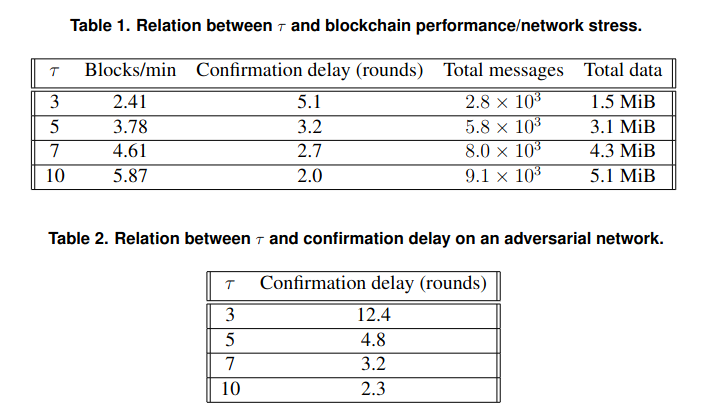
\includegraphics[width=\textwidth]{images/results.png}
\end{figure}
\end{frame}

\begin{frame}
Confirmação de blocos:
\begin{itemize}
    \item Baseada nos blocos que chegam até um nó
    \item O nó $i$ calcula, na rodada $x$, o número total de sorteios bem-sucedidos nos blocos que recebeu: $s_{i}^{x}$
    \item Se os outros peers na rede estão no mesmo fork que $i$, ele espera ver em média $\tau$ sorteios bem sucedidos por rodada
    \item Nó calcula o número de sorteios médio: $ \bar{s} = \frac{1}{\Delta_r} \sum s_i^x$
    \item Bloco confirmado quando $\bar{s}$ se torna suficientemente próximo de $\tau$
\end{itemize}
\end{frame}

\end{document}
